\section{Boxed Molecular Dynamics}

One of the recently proposed methods for simulating the thermodynamics and kinetics of rare events, boxed molecular dynamics \cite{Glowacki2009} (BXD), combines the advantages of two older methods: intramolecular diffusion dynamics theory\cite{Guo1999,Shalashilin1997} (IDDT) and molecular dynamics accelerated by phase space constraints\cite{Martinez-Nunez2006} (AXD).
In IDDT, the configuration space is sliced along a reaction coordinate and the diffusion coefficient is calculated using short MD simulations.
In AXD, the reactant configuration space is divided into two boxes. 
One box is placed close to the dividing surface representing the transition state ensemble and the other box represents the reactants.
In BXD, this approach is generalised to more boxes placed along the reaction coordinate.
The free energy profile is calculated from the flux ratios between the boxes.
BXD aims to efficiently simulate the dynamics of the process using the master equation with the rates calculated from the flux values.

\begin{figure}[h]
\label{fig:bxd-implement}
\centering
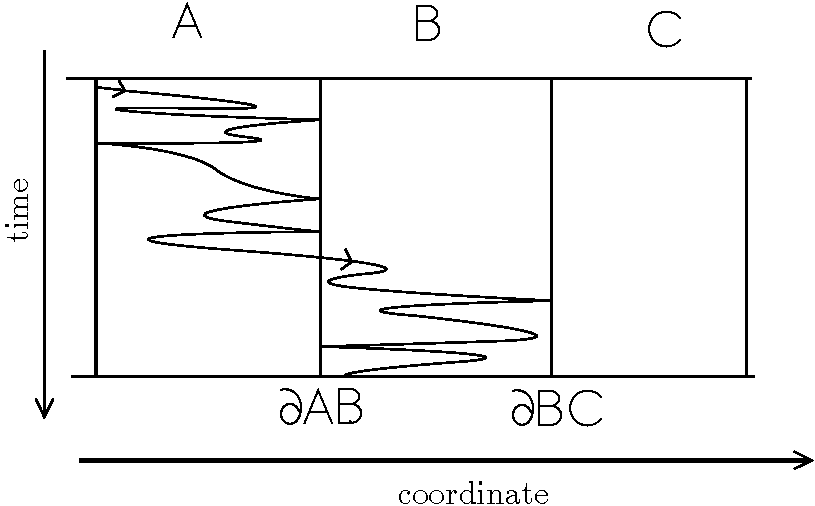
\includegraphics[width=9cm]{Images/bxdimplement.pdf}
\caption[Implementation of boxed molecular dynamics.]{Implementation of boxed molecular dynamics according to Glowacki {\it et al}.\cite{Glowacki2009} After a few (up to 30) inversion events, a hit from box A can be used for initialisation of the trajectory in box B. The method is not parallelised for the sake of easier initialisation of the trajectory in a box. }
\end{figure}

Implementation of BXD is straightforward.
An independent MD simulation is run in each box.
If the trajectory leaves the box, the positions are returned to the previous point of the simulation and a velocity inversion procedure is performed.
The projections of velocities onto the reaction coordinate are inverted while the velocity components parallel to the dividing surface remain unchanged.
The velocities of atoms not involved in the reaction coordinate are unchanged.
This inversion procedure does not change the energy, momentum or angular momentum.
The time of each inversion event is recorded.
The BXD trajectory in box i can be considered as an ensemble of $n_{\rm i-1}+n_{\rm i+1}$ subtrajectories, $n_{\rm i-1}$ being inverted from (ending at) the boundary between boxes i and i-1 and $n_{\rm i+1}$ from the boundary between boxes i and i+1.
The rate constant for the transition from box i to box i-1 is calculated from the simulation as the equilibrium flux:
\begin{equation}
\label{eq:eq-flux-simul}
k^{eq}_{\rm i \rightarrow i-1} = \frac{n_{\rm i-1}}{\sum_{j=1}^{n_{\rm i-1}} \tau_j} ~,
\end{equation}
where $\tau_j$ is the time length (evolution time) of the $j^{\rm th}$ trajectory inverted from the boundary between i and i-1.
The free energy difference between boxes i and i-1 is calculated from simulations in both boxes as:
\begin{equation}
\label{eq:bxd-fe}
\Delta G_{\rm i-1 \rightarrow i} = - k_B T \ln \left( \frac{k^{eq}_{\rm i-1 \rightarrow i}}{k^{eq}_{\rm i \rightarrow i-1}} \right) ~.
\end{equation}
Global dynamics can be described using the master equation with a tridiagonal transition matrix ${\bf A}$ with non-zero elements
\begin{equation}
\label{eq:bxd-A}
\begin{split}
A_{i,i-1} = k^{eq}_{\rm i-1 \rightarrow i} ~,
\\
A_{i,i} = - k^{eq}_{\rm i \rightarrow i-1} - k^{eq}_{\rm i \rightarrow i+1} ~,
\\
A_{i,i+1} = k^{eq}_{\rm i+1 \rightarrow i} ~.
\end{split}
\end{equation}

The authors explicitly state that the detailed balance condition must be satisfied and the dynamics must be ergodic for BXD to give correct results.
The BXD approach also assumes that the inversion procedure does not disturb the equilibrium distribution in the boxes.
An implicit assumption of BXD is that the TST rate constants can be used for transitions between neighbouring boxes.
However, the validity of these assumptions has not been tested separately.
The correctness of BXD as a whole is demonstrated by consistency of the results with ``brute force" MD and milestoning.
Free energy profiles have been shown to be robust with respect to box selection with fast convergence of the results with the number of subtrajectories $n_{\rm i-1}+n_{\rm i+1}$ sampled in each box i.


BXD was used to study conformational changes of small (10-13 amino acid) peptides.\cite{Glowacki2009}
The gain in computational efficiency was clearly demonstrated.
BXD has the potential to significantly decrease the computational cost of simulating the dynamics of rare events.
Firstly, slicing the reaction coordinate into boxes can significantly reduce the barrier height. 
Secondly, the independence of the simulations in the boxes makes parallelisation of the method trivial and formally correct.
Another advantage of the method is its natural relationship with the master equation.
BXD can be used for specialised applications, such as rationalisation of the power law dynamics of loop formation in a small peptide.\cite{Shalashilin2012}


A later paper\cite{Glowacki2011} by the same authors, which focused more on dynamics, suggested corrections for fast dynamical motion.
The distributions of FPT's differ from those obtained using milestoning and are not exponential.
The artificial increase in the number of short trajectories leads to overestimation of the calculated rate constants.
The authors suggest setting an evolution time threshold and excluding the trajectories below the threshold.
A more systematic correction of the rate constants would significantly improve the method.
Other important issues also have to be resolved.
The assumptions of BXD should be tested separately using simple models, and a method of error estimation should be developed.
Voronoi tesselation can be used to define the boxes instead of a reaction coordinate.\cite{Glowacki2011}
The method currently uses the Langevin equation, so it depends on an unphysical friction constant.
Using deterministic MD would systematically improve the description of the dynamics.
The present work attempts to benchmark and further develop BXD.

